\documentclass{beamer}

%%BEGIN HEADER
\usepackage{amsmath}
\usepackage{amssymb,amsthm,framed}
\usepackage{multirow,color,multicol}
\usepackage{fancyhdr,ifthen,lastpage}
\usepackage{verbatim,enumerate,cancel}
% --------------------------------------------------------------------
\newtheorem{thm}{Theorem}
\newtheorem{prop}{Proposition}

\theoremstyle{definition}
\newtheorem{defn}{Definition}
\newtheorem{fct}{Fact}

\theoremstyle{remark}
\newtheorem{remark}{Remark}

\newcommand{\Z}{\mathbb{Z}}
\newcommand{\C}{\mathbb{C}}
\newcommand{\Q}{\mathbb{Q}}
\newcommand{\N}{\mathbb{N}}
\newcommand{\R}{\mathbb{R}}
\newcommand{\B}{\mathcal{B}}
\renewcommand{\P}{\mathcal{P}}
\renewcommand{\L}{\mathcal{L}}
\newcommand{\F}{\mathbf{F}}
\newcommand{\x}{\mathbf{x}}
\newcommand{\y}{\mathbf{y}}

\newcommand{\sm}{\setminus}
\newcommand{\es}{\emptyset}
\newcommand{\ol}{\overline}
\newcommand{\inv}{^{-1}}
\newcommand{\seq}[1]{\{ {#1}_n\}}
\newcommand{\ds}{\displaystyle}
\newcommand{\mbf}{\mathbf}
\renewcommand{\=}{&=&}
\newcommand{\<}{\langle}
\renewcommand{\>}{\rangle}

\newcommand{\bmat}{\begin{bmatrix}}
\newcommand{\emat}{\end{bmatrix}}
\newcommand{\beq}{\begin{eqnarray*}}
\newcommand{\eeq}{\end{eqnarray*}}

\DeclareMathOperator{\repart}{Re}
\DeclareMathOperator{\impart}{Im}
\DeclareMathOperator{\Arg}{Arg}
\DeclareMathOperator{\trace}{tr}
\DeclareMathOperator{\rk}{rank}
\DeclareMathOperator{\nullsp}{null}
\DeclareMathOperator{\range}{range}
\DeclareMathOperator{\vspan}{span}
\DeclareMathOperator{\nullity}{nullity}
%%%%%END HEADER

%\usetheme{Berlin}
%\usecolortheme{orchid}

\setlength{\unitlength}{1mm}
 
\title{Lecture 9: Global Theory}
\author{Prof. Weiqing Gu}
\date{}
\institute{Math 142:\\Differential Geometry}

%--------------------
\begin{document}
%--------------------
\small

%----------
\begin{frame}
\titlepage
\end{frame}

%----------
\begin{frame}[t]
\frametitle{Global Theory}
\begin{enumerate}
\item Definitions\\
Closed Curve
\begin{itemize}
\item Simple
\item Nonsimple
\end{itemize}
Interior of a curve (region)
\begin{itemize}
\item Positively oriented
\item Negatively oriented
\end{itemize}

\item A formula to find the area of a region bounded by a curve

\item Solving the traditional Isoperimetric Problem
\end{enumerate}
\end{frame}

%----------
\begin{frame}[t]
\frametitle{Definitions and an Area Formula}
\begin{defn}
A \emph{differentiable function on a closed interval} $[a,b]$ is the restriction of a differentiable
function defined on an open interval containing $[a,b]$.
\end{defn}
\pause
\begin{defn}
A \emph{closed plane curve} is a regular parametrized curve $\alpha : [a,b] \to \R^2$ such that
$\alpha$ and all its derivatives agree at $a$ and $b$; that is,
\[ \alpha(a) = \alpha(b), \quad \alpha'(a) = \alpha'(b), \quad \alpha''(a) = \alpha''(b),\ldots \]
\pause
The curve $\alpha$ is \emph{simple} if it has no further self-intersections; that is, if $t_1, t_2 \in
[a,b)$, $t_1 \ne t_2$, then $\alpha(t_1) \ne \alpha(t_2)$.
\pause\vspace{1mm}

We usually consider the curve $\alpha : [0,\ell] \to \R^2$ parametrized by arc length $s$; hence,
$\ell$ is the length of $\alpha$. Sometimes we refer to a simple closed curve $C$, meaning the
trace of such an object. The curvature of $\alpha$ will be taken with a sign (see next slide).
\pause\vspace{1mm}

We assume that a \emph{simple closed curve} $C$ \emph{in the plane bounds a region of the
plane} that is called the \emph{interior} of $C$.
\end{defn}
\end{frame}

%----------
\begin{frame}[t]
\frametitle{Illustrations}
%\begin{center} 
\includegraphics[scale=0.5]{Fig1-20.pdf} 
%\end{center}
\end{frame}

%----------
\begin{frame}[t]
\frametitle{A Formula to Find the Area of a Region bounded by $C$}
\begin{block}{}
We shall make use of the following formula for the area $A$ bounded by a positively oriented
simple closed curve $\alpha(t) = (x(t),y(t))$, where $t \in [a,b]$ is an arbitrary parameter:
\[ A = - \int_a^b y(t) x'(t) \, dt = \int_a^b x(t) y'(t) \, dt = \frac{1}{2} \int_a^b (xy'-yx') \, dt. \]
\end{block}
\vspace{-1cm}
\begin{center}
\includegraphics[scale=0.6]{BoundedArea1.pdf} 
\includegraphics[scale=0.6]{BoundedArea2.pdf}
\end{center}
\end{frame}

%----------
\begin{frame}[t]
\frametitle{The Isoperimetric Problem}
\begin{block}{The Problem}
This is perhaps the oldest global theorem in differential geometry and is related to the following
(isoperimetric) problem. \emph{Of all simple closed curves in the plane with a given length $\ell$,
which one bounds the largest area?}
\end{block}
\pause
\begin{thm}[The Isoperimetric Inequality]
Let $C$ be a simple closed plane curve with length $\ell$, and let $A$ be the area of the region
bounded by $C$. Then
\[ \ell^2 - 4 \pi A \ge 0, \]
and equality holds if and only if $C$ is a circle.
\end{thm}
\end{frame}

%----------
\begin{frame}[t]
\frametitle{The Isoperimetric Inequality}
\begin{block}{Proof}
Let $E$ and $E'$ be two parallel lines which do not meet the closed curve $C$, and move them
together until they first meet $C$. We thus obtain two parallel tangent lines to $C$, $L$ and $L'$,
so that the curve is entirely contained in the strip bounded by $L$ and $L'$. Consider a circle
$S^1$ which is tangent to both $L$ and $L'$ and does not meet $C$. Let $O$ be the center of
$S^1$ and take a coordinate system with origin at $O$ and the $x$ axis perpendicular to $L$ and
$L'$.
\end{block}
\pause
\begin{picture}(100,20)
\only<2->{
	\put(40,-5){\includegraphics[scale=.075]{curve.pdf}}
	\put(50,11.5){\footnotesize $C$}
	}
	
\only<3>{
	\put(30,-22){\line(0,1){42}}
	\put(65.7,-22){\line(0,1){42}}
	\put(27.6,18){\scriptsize $L$}
	\put(66.4,18){\scriptsize $L'$}
	}
	
\only<4->{
	\put(40,-22){\line(0,1){42}}
	\put(55.7,-22){\line(0,1){42}}
	\put(37.6,18){\scriptsize $E$}
	\put(56.4,18){\scriptsize $E'$}
	}
	
\only<5->{
	\put(40,-22){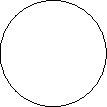
\includegraphics[scale=.87]{circle.pdf}}
	}
	
	\thinlines
	
\only<6->{
	\put(45,-14.15){\vector(1,0){14}}
	\put(47.85,-16){\vector(0,1){14}}
	\put(59.5, -14.5){\tiny $x$}
	\put(48.5,-2){\tiny $y$}
	}
\end{picture}
\end{frame}

%----------
\begin{frame}[t]
\frametitle{The Isoperimetric Inequality}
\begin{block}{Proof (cont'd)}
Parametrize $C$ by arc length, $\alpha(s) = (x(s), y(s))$, so that it is positively oriented and the
tangency points of $L$ and $L'$ are $s=0$ and $s=s_1$, respectively.
\vspace{1mm}

\uncover<3->{We can assume that the equation of $S_1$ is
\[ \ol \alpha(s) = (\ol x(s), \ol y(s)) = (x(s), \ol y(s)), s \in [0,\ell], \]
where $2r$ is the distance between $L$ and $L'$.}
\end{block}
\begin{picture}(100,20)
\only<1->{
	\put(40,-5){\includegraphics[scale=.075]{curve.pdf}}
	\put(50,11.5){\footnotesize $C$}
	\put(40,-22){\line(0,1){42}}
	\put(55.7,-22){\line(0,1){42}}
	\put(37.6,18){\scriptsize $E$}
	\put(56.4,18){\scriptsize $E'$}
	\put(40,-22){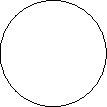
\includegraphics[scale=.87]{circle.pdf}}
	\thinlines
	\put(45,-14.15){\vector(1,0){14}}
	\put(47.85,-16){\vector(0,1){14}}
	\put(59.5, -14.5){\tiny $x$}
	\put(48.5,-2){\tiny $y$}
	}
	
\only<2->{
	\put(44,10){\tiny $\alpha$}
	}
	
\only<4->{
	\put(43,-20){\tiny $\ol \alpha$}
	\put(41,-7){\tiny $2r$}
	\put(40,-5.5){\line(1,0){15.7}}
	}
\end{picture}
\end{frame}

%----------
\begin{frame}[t]
\frametitle{Remarks}
\begin{remark}
It is easily checked that the above proof can be applied to $C^1$ \emph{curves}, that is, curves
$\alpha(t) = (x(t),y(t)),$ $t \in [a,b]$, for which we require only that the functions $x(t)$, $y(t)$ have
continuous first derivatives (which, of course, agree at $a$ and $b$ if the curve is closed).
\end{remark}
\pause
\begin{remark}
The isoperimetric inequality holds true for a wide class of curves. Direct proofs have been found
that work as long as we can define arc length and area for the curves under consideration. For the
applications, it is convenient to remark that the theorem holds for \emph{piecewise $C^1$ curves},
That is, continuous curves that are made up by a finite number of $C^1$ arcs. These curves
can have a finite number of corners, where the tangent is discontinuous.
\end{remark}
\end{frame}

%----------
\begin{frame}[t]
\frametitle{}

\end{frame}

%--------------------
\end{document}
%--------------------